\section{System Overview}
Our system mainly consists of a set of processes which receive events, process them and forward to next processes. We use the term adapters for special processes which receive events from out side systems. These processes and adapters forms a graph which represents the way a given event stream being processed within the system. Rest of this section further describes this concept at a user level. In the next section we provide a detail explanation about how we have make this interprocess communication efficient.
\subsection{Process Graph}
A Process graph (Figure \ref{processgraph}) mainly consists of the adapters, processes which does the processing logic and their interaction patterns. Adapters receive events from out side systems and forward them to other processes. Processes process events according to a given logic and emits the generated events either to processes or out side systems. 

\begin{figure}[!t]
	\centering
	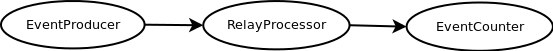
\includegraphics[width=3.0in]{processgraph.png}
	\caption{Process Graph}
	\label{processgraph}
\end{figure}

\subsection{Runtime Graph}
When the system is deployed, there can be many instances of one process to handle higher loads making system scalable. Figure \ref{runtimegraph} shows possible runtime graph for above process graph. Here each parent process instance sends events to two child process instances. However in this case parent process instance has to pick a child process instance to send the message as well. One way of handling this problem is to pick a random node. Other way is to send messages with same key to same child process instance. 

\begin{figure}[!t]
        \centering
        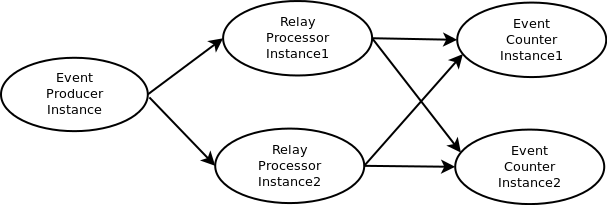
\includegraphics[width=3.0in]{runtimegraph.png}
        \caption{Runtime Graph}
        \label{runtimegraph}
\end{figure}

\subsection{Specifying the Runtime Graph}

A runtime graph mainly consists of a set of processes, adapters and events. Processes, adapters and events can be created by implementing respective interfaces as shown below.

\definecolor{dkgreen}{rgb}{0,0.6,0}
\definecolor{gray}{rgb}{0.5,0.5,0.5}
\definecolor{mauve}{rgb}{0.58,0,0.82}

\lstset{frame=tb,
  language=Java,
  aboveskip=3mm,
  belowskip=3mm,
  showstringspaces=false,
  columns=flexible,
  basicstyle={\small\ttfamily},
  numbers=none,
  numberstyle=\tiny\color{gray},
  keywordstyle=\color{blue},
  commentstyle=\color{dkgreen},
  stringstyle=\color{mauve},
  breaklines=true,
  breakatwhitespace=true,    
  tabsize=2
}

\begin{lstlisting}
public interface Event {
    public String getKey();
    public void serialize(DataOutput dataOutput);
    public void parse(DataInput dataInput);
}

public interface Element {
    public void initialise(Container container,
                     Map<String,String> parameters);
}

public interface Adaptor extends Element {
    public void start();
}

public interface Processor extends Element {
    public void onEvent(Event event);
}
\end{lstlisting}

 The Event interface has a method to get the key for a given event. This key is used in sending messages to next processes as described earlier. Parse and serialize methods of event interface are used to direcly serialize the object state to underline streams. Process interface has a method called onEvent which underline framework invokes when it receives an event to that process. The start method of the adapter interace is invoked by the framework and that can be used to pull events from out side systems onces the system starts. At the initilization time both processes and adapters receive the container object which can be used to send events to other processes. Users can specify the runtime graph to the system using a json file as shown below. 

\lstinputlisting{runtimegraph.json}

\subsection{Deployment}

A deployment of the system consists of a manager node and a set of worker nodes \ref{deployment}. Worker nodes are grouped in to clusters so that at the runtime graph users can specify to which clusters each processes needs to get deployed. Once the system starts worker nodes communicate with each other passing messages.

\begin{figure}[!t]
        \centering
        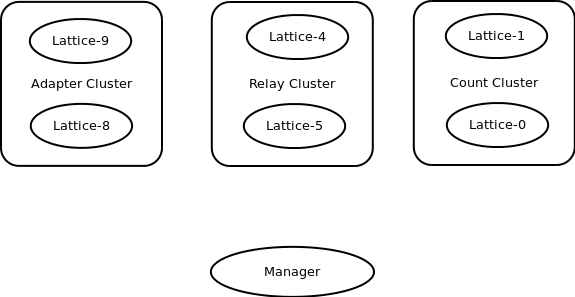
\includegraphics[width=3.0in]{deployment.png}
        \caption{Deployment}
        \label{deployment}
\end{figure}



 
